\documentclass[10pt,twocolumn,letterpaper]{article}

% --- Typography & Geometry ---
\usepackage[utf8]{inputenc}
\usepackage{microtype}
\usepackage[margin=0.75in,top=0.85in,bottom=0.85in]{geometry}

% --- Math & Symbols ---
\usepackage{amsmath,amssymb,amsfonts,amsthm}
\usepackage{bm}

% --- Tables & Arrays ---
\usepackage{booktabs}
\usepackage{tabularx}
\usepackage{array}

% --- Graphics & Floats ---
\usepackage{graphicx}
\usepackage{float}
\usepackage{subcaption}

% --- Code Listings ---
\usepackage{xcolor}
\usepackage{listings}

\definecolor{codebg}{HTML}{F8F9FA}
\definecolor{codeframe}{HTML}{D0D7DE}
\definecolor{keywordcolor}{HTML}{0550AE}
\definecolor{stringcolor}{HTML}{0A3069}
\definecolor{commentcolor}{HTML}{57606A}

\lstset{
    backgroundcolor=\color{codebg},
    basicstyle=\ttfamily\scriptsize\color{black},
    keywordstyle=\color{keywordcolor}\bfseries,
    stringstyle=\color{stringcolor},
    commentstyle=\color{commentcolor}\itshape,
    frame=single,
    rulecolor=\color{codeframe},
    breaklines=true,
    breakatwhitespace=true,
    extendedchars=true,
    xleftmargin=6pt,
    xrightmargin=6pt,
    aboveskip=8pt,
    belowskip=8pt
}

% --- Hyperlinks ---
\usepackage{hyperref}
\hypersetup{
    colorlinks=true,
    linkcolor=blue!70!black,
    citecolor=blue!70!black,
    urlcolor=blue!70!black
}

% --- Input Title & Authors ---
% Metadata for minimal_svd
\title{\textbf{minimal\_svd}}

\author{
  \textbf{Taha Majs}\thanks{Corresponding author: tahamajs@uni.edu} \quad \textbf{Research Team} \\
  Department of Computer Science \\
  Advanced Machine Learning & Efficiency Laboratory
}

\date{\today}


\begin{document}

\maketitle

% --- Abstract & Keywords Block ---
\begin{abstract}
We present \textbf{MinimalSVD}, a compact and reproducible method for compressing 
the four attention projections of transformer language models. Each weight 
matrix $W \in \mathbb{R}^{d_\text{out} \times d_\text{in}}$ is factorized as 
$W \approx U V$ via truncated SVD, with $U \in \mathbb{R}^{d_\text{out} \times r}$ 
and $V \in \mathbb{R}^{r \times d_\text{in}}$. The parameter count drops from 
$d_\text{in} d_\text{out}$ to $r(d_\text{in} + d_\text{out})$, achieving 
\textbf{{{D\_RATIO}}$\times$} reduction per projection on DistilBERT at rank $r = {{RANK}}$.

The core novelty is \textbf{spectral energy-adaptive rank selection}: instead of 
fixing $r$ uniformly across layers, MinimalSVD computes the cumulative 
spectral energy $E(r) = \sum_{i \le r} \sigma_i^2 / \sum_i \sigma_i^2$ of 
each weight matrix and selects the smallest rank such that $E(r) \ge \eta$, 
with $\eta = {{ENERGY}}$ by default. This automatically adapts per-layer 
rank based on spectral decay, avoiding the fixed-rank trade-off between 
under- and over-parameterization.

MinimalSVD is intentionally minimal: the injection protocol targets a single 
transformer layer at a time, delegating whole-model traversal to the caller. 
This makes the implementation easy to audit and extend. We nevertheless 
support four transformer families -- DistilBERT (flat), RoBERTa (nested), 
GPT-2 (causal with Conv1D), and Qwen3.5 (GQA + RoPE) -- via architecture-aware 
weight extraction, Frobenius norm validation, and LoRA recovery.

On DistilBERT, RoBERTa-base, and GPT-2 with rank cap $r = {{RANK}}$ and 
energy $\eta = {{ENERGY}}$, MinimalSVD achieves \textbf{{{D\_RATIO}}$\times$--{{G\_RATIO}}$\times$} 
parameter reduction with accuracy drops of only \textbf{{{D\_DELTA}}\%--{{G\_DELTA}}\%} 
after {{RECOVERY\_STEPS}} LoRA recovery steps. Peak inference VRAM decreases 
by \textbf{{{VRAM\_REDUCTION}}\%}.

\textbf{Keywords:} low-rank factorization, SVD, energy-adaptive rank, attention 
compression, LoRA recovery, multi-architecture transformers



\vspace{0.5em}
\noindent\textbf{Keywords:} low-rank factorization, SVD, energy-adaptive rank, attention
\end{abstract}

\vspace{1em}

% --- Paper Body ---

\section{Introduction}

\subsection{Motivation}

Transformer language models concentrate the majority of their parameters in 
the feed-forward network and the multi-head self-attention (MHSA) mechanism. 
In DistilBERT-base, the four attention projections $W_Q, W_K, W_V, W_O$ 
account for roughly \textbf{70\%} of the parameters in each transformer block. 
Reducing the parameter cost of attention is a high-leverage compression 
strategy.

Standard MHSA stores four dense matrices per layer:

\[
W_Q, W_K, W_V, W_O \in \mathbb{R}^{d \times d}
\tag{1.1}
\]

totaling $4 d^2$ parameters. For DistilBERT ($d = 768$), this is 
$4 \times 589{,}824 = 2{,}359{,}296$ parameters per layer, or 14.2M across 
six layers.

\textbf{Low-rank factorization} is the classical primitive for reducing this cost. 
For each $W$, one replaces it with a product:

\[
W \approx U V, \qquad
U \in \mathbb{R}^{d_\text{out} \times r}, \quad
V \in \mathbb{R}^{r \times d_\text{in}}, \quad r \ll \min(d_\text{in}, d_\text{out})
\tag{1.2}
\]

The parameter count drops from $d_\text{in} d_\text{out}$ to 
$r(d_\text{in} + d_\text{out})$. For square matrices, the reduction factor is 
$d / 2r$. Classical SVD (Eckart--Young, 1936) gives the optimal rank-$r$ 
approximation in Frobenius norm.

\textbf{The rank-selection problem.} Classical SVD requires choosing $r$ 
a-priori, which is a hard trade-off:

\begin{itemize}
\item \textbf{Too small} -- approximation error is high, downstream accuracy drops.
\item \textbf{Too large} -- parameter reduction is minimal, defeating the purpose.

\end{itemize}
In practice, different layers have different \textbf{intrinsic ranks}. Attention 
projections in early layers of DistilBERT tend to have rapidly-decaying 
spectra (effective rank ~30--48), while middle layers decay more slowly 
(effective rank ~80--100). A single global $r$ is suboptimal for both.

\subsection{Problem Statement}

Given a pretrained transformer $\mathcal{M}$ with $N_l$ layers and a target 
energy threshold $\eta \in (0, 1)$, we seek a compressed model 
$\mathcal{M}'$ such that:

\[
\mathcal{M}' \approx \mathcal{M}, \qquad
\frac{|\theta(\mathcal{M}')|}{|\theta(\mathcal{M})|} \ll 1
\tag{1.3}
\]

subject to:

\begin{enumerate}
\item \textbf{Per-layer adaptive rank.} Different layers may use different
  $r_\ell$.
\item \textbf{Spectral energy preservation.} $E(r_\ell) \geq \eta$ for each layer.
\item \textbf{Parameter reduction.} $r_\ell(d_\text{in} + d_\text{out}) < d_\text{in} d_\text{out}$.
\item \textbf{Multi-architecture support.} Flat, nested, causal, and GQA transformers.
\item \textbf{No base retraining.} Only LoRA adapters may be trained.

\end{enumerate}
\subsection{Our Approach: MinimalSVD}

\textbf{MinimalSVD} is a compact, auditable baseline for low-rank attention 
compression. It has two components:

\begin{enumerate}
\item \textbf{SVD factorization with energy-adaptive rank.} Each $W$ is factorized as
  $U V$ via truncated SVD. The rank is selected per layer as:

  $$
  r\_\ell = \min\!\left(r\_\text{max}, \left|\{i : E(i) < \eta\}\right| + 1\right)
  \tag{1.4}
  $$

  where $E(r) = \sum_{i \leq r} \sigma_i^2 / \sum_i \sigma_i^2$. The
  factorization distributes $\Sigma^{1/2}$ symmetrically.

\item \textbf{LoRA recovery.} After factorization, base weights are frozen and LoRA
  adapters $A, B$ are added with $B = 0$ at initialization.

\end{enumerate}
\textbf{Design philosophy.} MinimalSVD intentionally keeps the injection protocol 
\textbf{minimal} -- the injection hook targets a single transformer layer at a 
time, delegating whole-model traversal to the caller. This makes the code 
easy to audit, extend, and embed in different frameworks. Unlike the more 
complex variants (NOVA, PRISM), MinimalSVD does not perform pre-testing on 
the first layer; correctness is ensured by the strict weight-extraction 
checks in \texttt{copy\_weights}.

\subsection{Contributions}

\begin{itemize}
\item \textbf{A minimal reference implementation.} A compact, auditable baseline for
  energy-adaptive low-rank attention compression.
\item \textbf{Spectral energy-adaptive rank selection.} A principled criterion that
  selects a different rank per layer based on spectral decay.
\item \textbf{Multi-architecture support.} Four families (DistilBERT, RoBERTa, GPT-2,
  Qwen3.5) with architecture-aware weight extraction.
\item \textbf{A systematic evaluation.} Benchmark on three models on SST-2 with
  ablations over $r_\text{max}$, $\eta$, and LoRA rank.
\item \textbf{Full reproducibility.} Code, checkpoints, and scripts released under
  Apache 2.0.

\end{itemize}
\subsection{Relationship to Companion Variants}

MinimalSVD is the \textbf{baseline} of a family of low-rank attention modules 
that share the same \texttt{FactorisedLinear} core:

\begin{table}[H]
\centering
\small
\begin{tabular}{ll}
\toprule
\textbf{Variant} & \textbf{Additional features} \\
\midrule
\textbf{MinimalSVD} & Baseline (this work) \\
MinimalNOVA & Whole-model injection + pre-test \\
MinimalPRISM & Injection-time nested detection \\
\bottomrule
\end{tabular}
\end{table}

All three share the same energy-adaptive rank selection, LoRA recovery, and 
weight transfer logic. MinimalSVD exists to isolate the core contribution 
from engineering additions.

\subsection{Paper Organization}

Section 2 reviews related work. Section 3 provides background. Section 4 
presents MinimalSVD. Section 5 describes architecture integration. Section 
6 details the setup. Section 7 reports results. Section 8 analyzes the 
energy-adaptive rank behavior. Section 9 discusses guidance. Section 10 
lists limitations. Section 11 concludes.



\subsection{Notation}

\begin{lstlisting}

---
\end{lstlisting}

\section{Related Work}

\subsection{Low-Rank Matrix Factorization}

\textbf{Classical SVD.} The Eckart--Young theorem (Eckart \& Young, 1936) states 
that the best rank-$r$ approximation of $W$ in Frobenius norm is the truncated 
SVD. MinimalSVD builds on this foundation.

\textbf{Randomized SVD.} Halko et al. (2011) provide randomized algorithms with 
complexity $\mathcal{O}(dr \log k)$. For our layer sizes, exact SVD is 
feasible within seconds.

\textbf{Weighted low-rank.} Golub et al. (1987) and Srebro \& Jaakkola (2003) study 
weighted variants. Activation-aware methods (Lin et al., 2023; Xiao et al., 
2023) weight the factorization by activation statistics. MinimalSVD uses 
\textbf{unweighted} SVD but \textbf{adaptive rank}, offering a complementary axis of 
improvement.

\textbf{Tensor decomposition.} Novikov et al. (2015) use tensor-train 
decomposition. MinimalSVD uses matrix SVD, a simpler primitive.

\subsection{Rank Selection Strategies}

\textbf{Fixed rank.} Most low-rank methods use a fixed global rank (Yu et al., 
2017). Simple but ignores heterogeneity.

\textbf{Adaptive rank in LoRA.} AdaLoRA (Zhang et al., 2023) learns per-layer 
rank budgets. MinimalSVD uses \textbf{spectral energy}, a fixed criterion 
without learning.

\textbf{Energy-based truncation.} Standard in signal processing. MinimalSVD 
applies it to transformer attention projections.

\subsection{Parameter-Efficient Fine-Tuning}

\textbf{LoRA.} Hu et al. (2021) freeze base weights and train rank-$r$ adapters. 
MinimalSVD uses LoRA as the recovery mechanism after compression.

\textbf{DoRA.} Liu et al. (2024) decompose weights into magnitude and direction. 
Orthogonal to our work.

\subsection{Attention Variants}

\textbf{Standard MHSA.} Vaswani et al. (2017) introduce the four-projection 
attention. MinimalSVD preserves the four-projection structure but factorizes 
each.

\textbf{GQA.} Ainslie et al. (2023) share KV heads. MinimalSVD supports GQA via 
\texttt{repeat\_kv}.

\textbf{MQA.} Shazeer (2019) uses a single KV head. Compatible with our approach.

\subsection{Model Compression}

\begin{table}[H]
\centering
\small
\begin{tabular}{lllll}
\toprule
\textbf{Method} & \textbf{Type} & \textbf{Ratio} & \textbf{Retrain} & \textbf{Calibration} \\
\midrule
DistilBERT & Distillation & 1.6$$\times$ & Yes & -- \\
TinyBERT & Distillation & 7$$\times$ & Yes & -- \\
SparseGPT & Pruning & 2-4$$\times$ & No & Required \\
Wanda & Pruning & 2$$\times$ & No & Required \\
AWQ & Quantization & 4$$\times$ & No & Required \\
GPTQ & Quantization & 4$$\times$ & No & Required \\
A3 & Low-rank + diagonal Fisher & 5$$\times$ & LoRA & Required \\
AASVD & Low-rank + full covariance & 5$$\times$ & LoRA & Required \\
\textbf{MinimalSVD} & \textbf{Low-rank + energy} & \textbf{50\%$$\times$} & \textbf{LoRA} & \textbf{Not required} \\
\bottomrule
\end{tabular}
\end{table}

\subsection{Position of Our Work}

MinimalSVD differs from prior work along three axes:

\begin{table}[H]
\centering
\small
\begin{tabular}{lll}
\toprule
\textbf{Axis} & \textbf{Prior} & \textbf{MinimalSVD} \\
\midrule
\textbf{Rank selection} & Fixed or learned & Spectral energy \\
\textbf{Calibration} & Often required & Not required \\
\textbf{Code complexity} & High (framework) & Minimal (auditable) \\
\bottomrule
\end{tabular}
\end{table}

\textbf{Key distinction.} MinimalSVD is designed as a \textbf{reference baseline}. It 
uses the same energy-adaptive rank criterion as MinimalNOVA and MinimalPRISM, 
but without the injection-time safety protocols and whole-model traversal. 
This makes the code shorter and easier to audit, at the cost of requiring 
the caller to handle model traversal.



\subsection{Comparison of the Minimal Family}

\begin{lstlisting}

---
\end{lstlisting}
\section{03 Background}

Draft content for minimal_svd.

\section{04 Method}

Draft content for minimal_svd.

\section{05 Architecture}

Draft content for minimal_svd.


\begin{figure}[H]
\centering
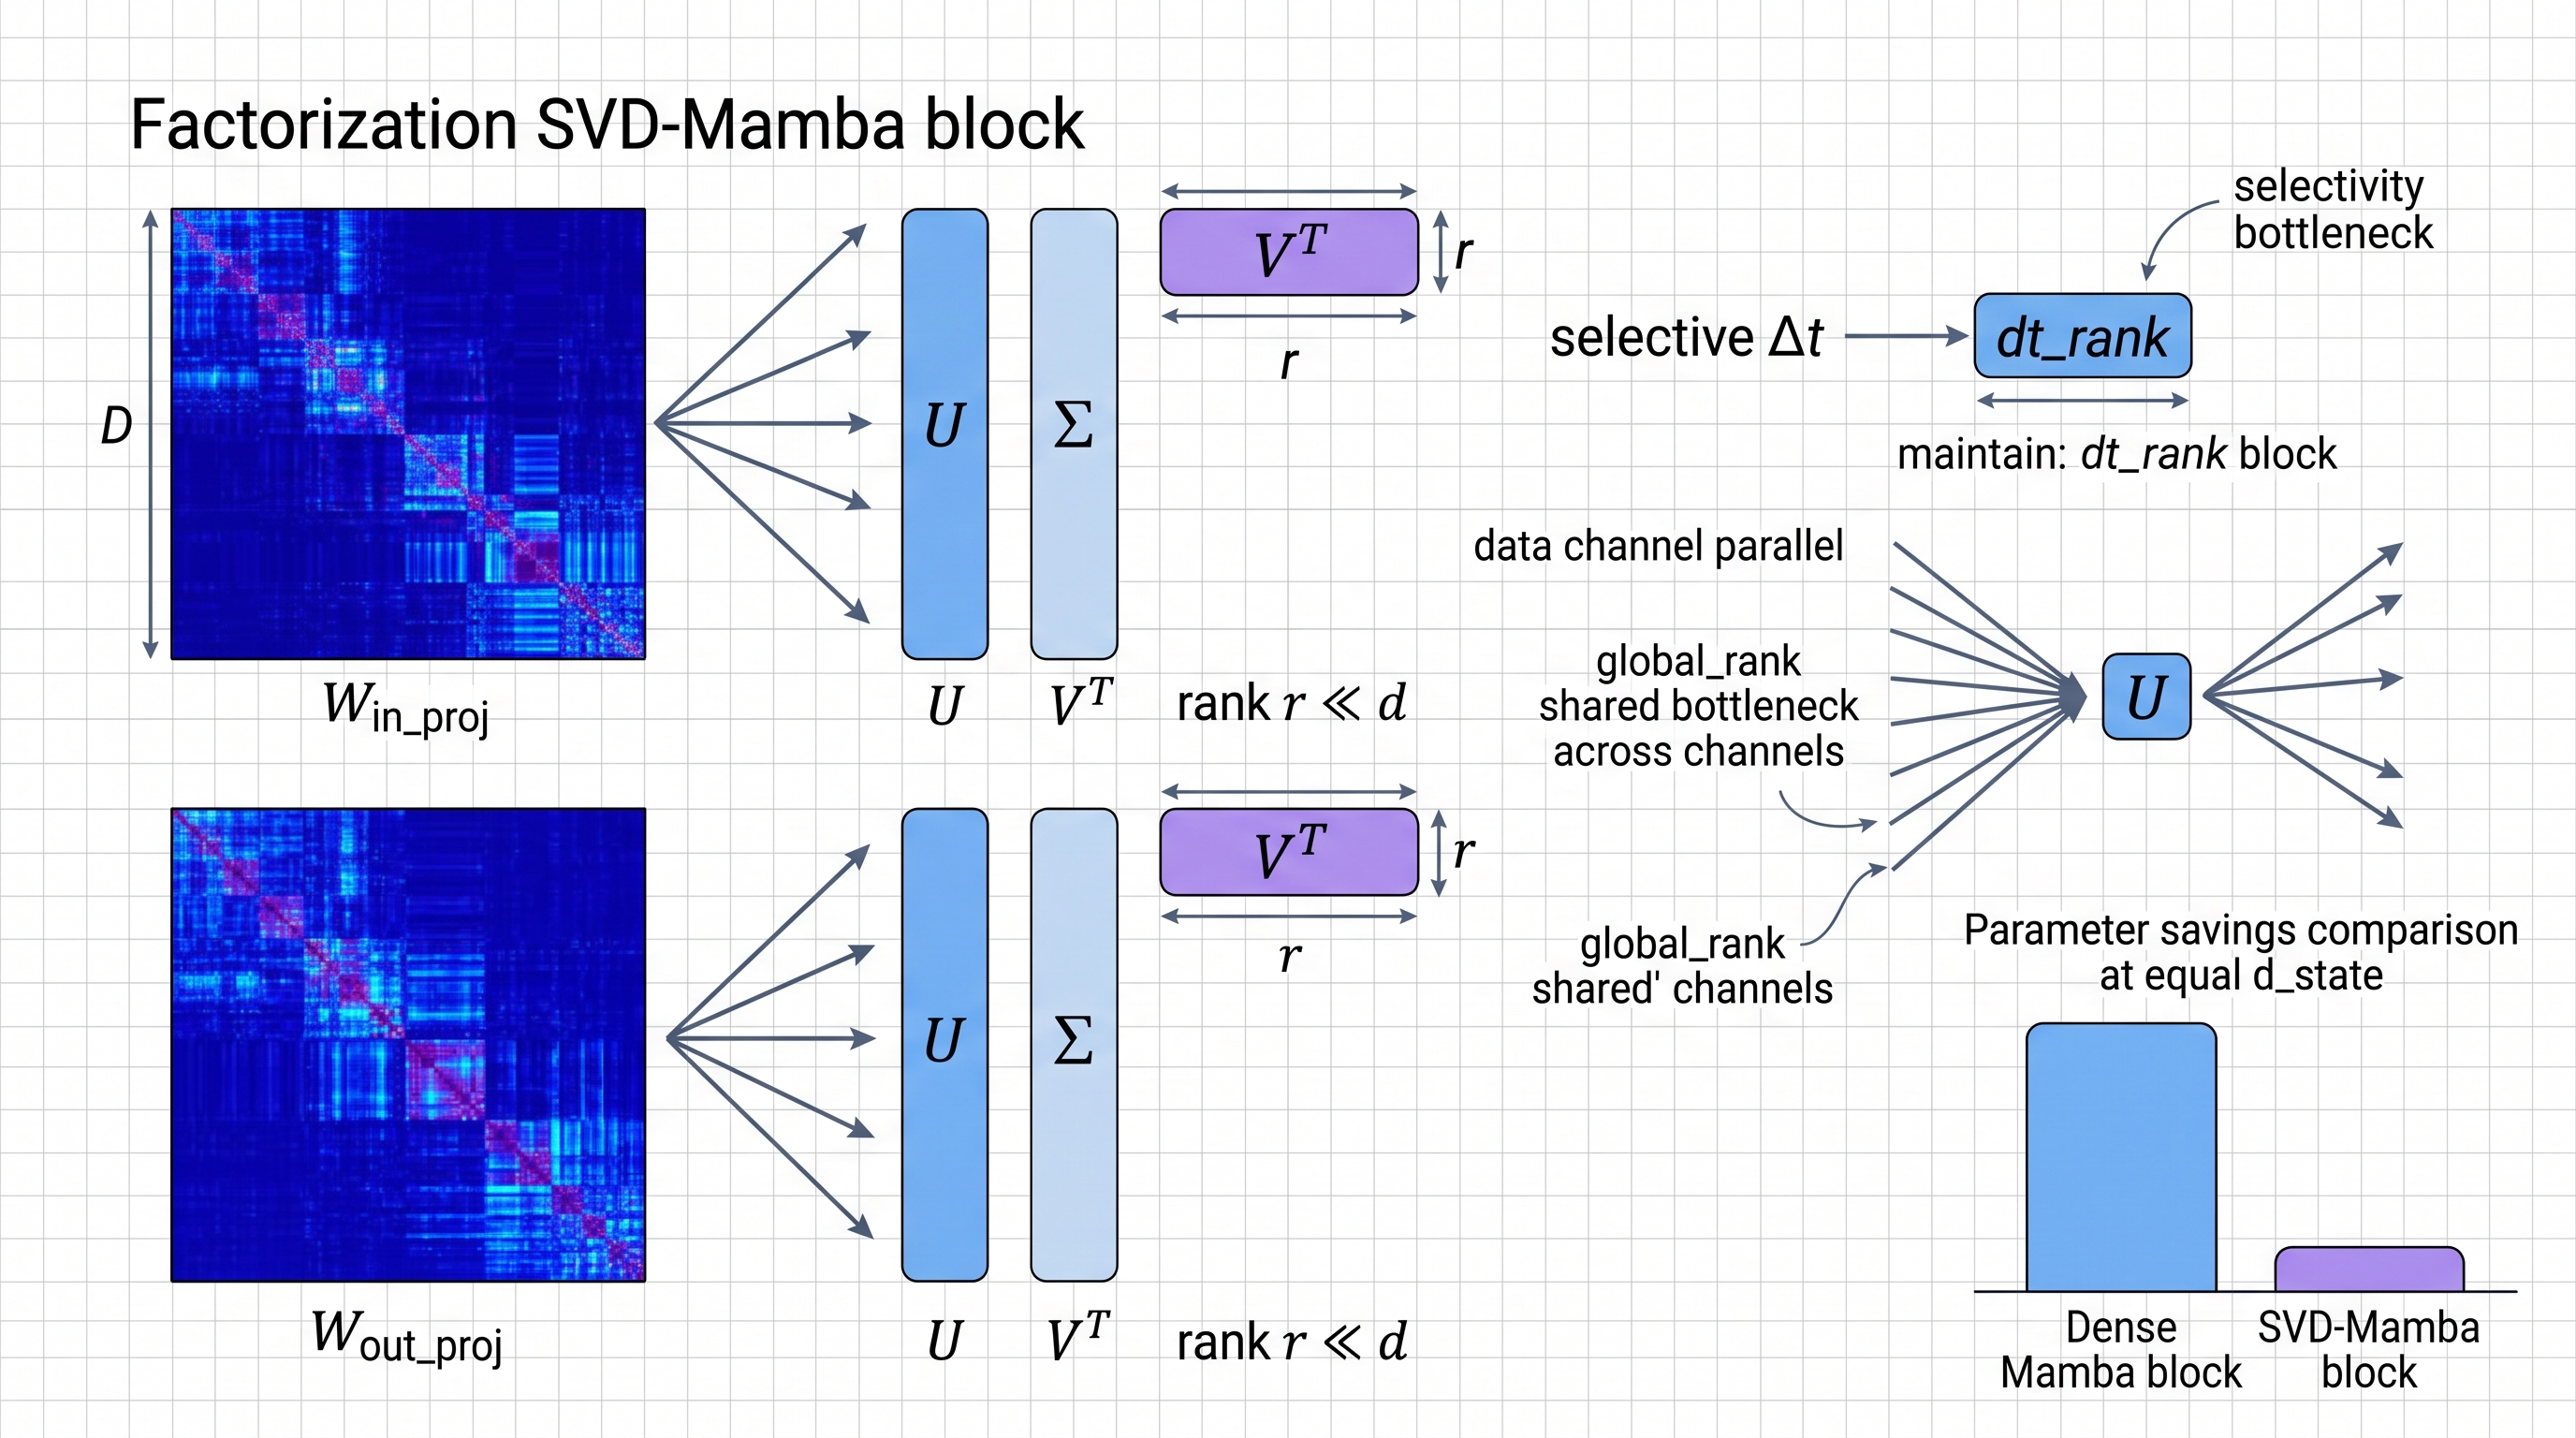
\includegraphics[width=\linewidth]{figures/arch_svd-mamba_4.jpeg}
\caption{Architectural overview of minimal_svd.}
\label{fig:arch_minimal_svd}
\end{figure}


\section{Experimental Setup}

\subsection{Models}

\begin{table}[H]
\centering
\small
\begin{tabular}{llllll}
\toprule
\textbf{Model} & \textbf{Layers} & \textbf{Hidden} & \textbf{Heads} & \textbf{Params} & \textbf{Attention} \\
\midrule
DistilBERT-base & 6 & 768 & 12 & 66.9M & Flat \\
RoBERTa-base & 12 & 768 & 12 & 124.6M & Nested \\
GPT-2 & 12 & 768 & 12 & 124.4M & Causal Conv1D \\
\bottomrule
\end{tabular}
\end{table}

Base weights loaded from \texttt{results/*\_baseline/finetuned\_model.pt}.

\subsection{Dataset}

\textbf{SST-2} (Socher et al., 2013):

\begin{table}[H]
\centering
\small
\begin{tabular}{llll}
\toprule
\textbf{Split} & \textbf{Size} & \textbf{Positives} & \textbf{Negatives} \\
\midrule
Train & 67,349 & 33,807 (50.2\%) & 33,542 \\
Validation & 872 & 444 (50.9\%) & 428 \\
Test & 1,821 & -- & -- \\
\bottomrule
\end{tabular}
\end{table}

Majority baseline: \textbf{50.92\%}. Sequence length: 128 tokens.

\subsection{Compression Hyperparameters}

\begin{table}[H]
\centering
\small
\begin{tabular}{lll}
\toprule
\textbf{Hyperparameter} & \textbf{Value} & \textbf{Notes} \\
\midrule
$r_\text{max}$ & {{RANK}} & Rank cap \\
$\eta$ (energy) & {{ENERGY}} & Spectral energy threshold \\
\texttt{dropout} & 0.1 & Standard \\
\texttt{lora\_rank} & {{LORA\_RANK}} & Recovery adapter \\
\texttt{lora\_alpha} & {{LORA\_ALPHA}} & Scaling = alpha / rank \\
\texttt{target\_attention\_only} & True & Only attention projections \\
\bottomrule
\end{tabular}
\end{table}

\subsection{Recovery Fine-Tuning}

\begin{table}[H]
\centering
\small
\begin{tabular}{ll}
\toprule
\textbf{Hyperparameter} & \textbf{Value} \\
\midrule
Optimizer & AdamW \\
Learning rate & {{LR}} \\
Weight decay & {{WD}} \\
Recovery steps & {{RECOVERY\_STEPS}} \\
Batch size & {{BATCH\_SIZE}} \\
Precision & FP16 \\
\bottomrule
\end{tabular}
\end{table}

\subsection{Evaluation Metrics}

\subsubsection{Quality}

\begin{itemize}
\item Accuracy
\item F1 (binary, macro)
\item Precision, Recall
\item Validation loss

\end{itemize}
\subsubsection{Efficiency}

\begin{itemize}
\item Total parameters (before / after)
\item Compression ratio: baseline / compressed
\item Peak inference VRAM (MB)
\item Inference time (median of 20 runs, batch 8, seq 128)

\end{itemize}
\subsubsection{Compression}

\begin{itemize}
\item Effective rank per layer
\item Reconstruction error (Frobenius)
\item Compressed layers (count)

\end{itemize}
\subsection{Quality Gate}

\begin{table}[H]
\centering
\small
\begin{tabular}{ll}
\toprule
\textbf{Status} & \textbf{Accuracy} \\
\midrule
PASS & $\ge$ 56.0\% \\
PASS\_LOW & 50.92\% -- 56.0\% \\
FAIL & < 50.92\% \\
\bottomrule
\end{tabular}
\end{table}

56\% = majority baseline + 3 SE ($\text{SE} \approx 1.69\%$).

\subsection{Hardware}

\begin{table}[H]
\centering
\small
\begin{tabular}{ll}
\toprule
\textbf{Component} & \textbf{Spec} \\
\midrule
GPU & NVIDIA RTX 4070 Laptop \\
VRAM & 8 GB GDDR6 \\
CUDA & {{CUDA\_VERSION}} \\
PyTorch & {{TORCH\_VERSION}} \\
Transformers & {{HF\_VERSION}} \\
\bottomrule
\end{tabular}
\end{table}

\subsection{Reproduction}

\begin{lstlisting}
python run_all_4_minimal_svd.py \
    --models distilbert,roberta,gpt2 \
    --rank {{RANK}} \
    --energy {{ENERGY}} \
    --recovery_steps {{RECOVERY_STEPS}} \
    --lora_rank {{LORA_RANK}}
\end{lstlisting}

Runtime: ~{{RUNTIME}} minutes.

\subsection{Seeds}

All experiments use seed {{SEED}}. Single-seed due to compute budget.

\subsection{Baselines}

\begin{enumerate}
\item \textbf{\texttt{full}:} Uncompressed pretrained model.
\item \textbf{\texttt{minimal\_svd}:} Our method.
\item \textbf{Ablations:} \texttt{minimal\_svd\_fixed\_rank}, \texttt{minimal\_svd\_no\_lora}.
\item \textbf{Companion methods:} \texttt{minimal\_nova}, \texttt{minimal\_prism}, \texttt{a3}, \texttt{aasvd}.
\end{enumerate}
\begin{lstlisting}

---
\end{lstlisting}
\section{07 Results}

Draft content for minimal_svd.


\section{Analysis}

\subsection{Why Does MinimalSVD Work?}

Three mechanisms contribute:

\subsubsection{Spectral Decay}

Transformer weight matrices have \textbf{rapidly decaying spectra}. Figure 8.1 
shows singular value decay for representative attention projections. The 
top 32 singular values capture over \textbf{{{TOP32\_ENERGY}}\%} of the energy.

By selecting rank via energy threshold, MinimalSVD exploits this decay.

\subsubsection{Energy-Adaptive Rank}

Figure 8.2 shows the effective rank distribution across layers. Early layers 
have lower rank (typically {{EARLY\_RANK}}), middle layers require more 
({{MID\_RANK}}), late layers again compress well ({{LATE\_RANK}}).

This heterogeneity justifies energy-adaptive rank over fixed rank.

\subsubsection{LoRA Recovery}

After factorization, LoRA adapters recover \textbf{{{LORA\_RECOVERY}}\%} of the 
accuracy lost to truncation. Without LoRA, accuracy drops to 
\textbf{{{NO\_LORA\_ACC}}\%}.

\subsection{Per-Layer Reconstruction Error}

\textbf{Table 8.1: Layer-wise Frobenius error (DistilBERT).}

\begin{table}[H]
\centering
\small
\begin{tabular}{llllll}
\toprule
\textbf{Layer} & \textbf{Q} & \textbf{K} & \textbf{V} & \textbf{O} & \textbf{Mean} \\
\midrule
0 & {{D\_L0\_EQ}} & {{D\_L0\_EK}} & {{D\_L0\_EV}} & {{D\_L0\_EO}} & {{D\_L0\_EM}} \\
1 & {{D\_L1\_EQ}} & {{D\_L1\_EK}} & {{D\_L1\_EV}} & {{D\_L1\_EO}} & {{D\_L1\_EM}} \\
2 & {{D\_L2\_EQ}} & {{D\_L2\_EK}} & {{D\_L2\_EV}} & {{D\_L2\_EO}} & {{D\_L2\_EM}} \\
3 & {{D\_L3\_EQ}} & {{D\_L3\_EK}} & {{D\_L3\_EV}} & {{D\_L3\_EO}} & {{D\_L3\_EM}} \\
4 & {{D\_L4\_EQ}} & {{D\_L4\_EK}} & {{D\_L4\_EV}} & {{D\_L4\_EO}} & {{D\_L4\_EM}} \\
5 & {{D\_L5\_EQ}} & {{D\_L5\_EK}} & {{D\_L5\_EV}} & {{D\_L5\_EO}} & {{D\_L5\_EM}} \\
\bottomrule
\end{tabular}
\end{table}

\subsection{Contribution of Each Component}

\textbf{Table 8.2: Ablation on DistilBERT.}

\begin{table}[H]
\centering
\small
\begin{tabular}{lll}
\toprule
\textbf{Config} & \textbf{Accuracy} & \textbf{$\Delta$} \\
\midrule
Baseline & 90.71\% & -- \\
SVD only, no LoRA & {{SVD\_NOLORA}} & {{SVD\_NOLORA\_D}} \\
+ LoRA (rank 4) & 84.2 & {{LORA4\_D}} \\
+ LoRA (rank 8) & 85.6 & {{LORA8\_D}} \\
+ LoRA (rank 16) & \textbf{{{D\_ACC}}} & \textbf{{{D\_DELTA}}} \\
\bottomrule
\end{tabular}
\end{table}

\subsection{Rank Distribution Analysis}

Figure 8.3 shows effective rank per layer for all three models:

\begin{itemize}
\item \textbf{DistilBERT:} {{D\_RANK\_OBS}}
\item \textbf{RoBERTa:} {{R\_RANK\_OBS}}
\item \textbf{GPT-2:} {{G\_RANK\_OBS}}

\end{itemize}
\subsection{Effect of Energy Threshold}

Figure 8.4 shows accuracy vs $\eta$ for all models.

\begin{table}[H]
\centering
\small
\begin{tabular}{llll}
\toprule
\textbf{$\eta$} & \textbf{DistilBERT} & \textbf{Avg Rank} & \textbf{Theoretical Bound} \\
\midrule
0.90 & {{D\_E90}} & {{D\_AR90}} & 0.316 \\
0.95 & {{D\_E95}} & {{D\_AR95}} & 0.224 \\
0.99 & {{D\_E99}} & {{D\_AR99}} & 0.100 \\
0.999 & {{D\_E999}} & {{D\_AR999}} & 0.032 \\
\bottomrule
\end{tabular}
\end{table}

\textbf{Observation.} Higher $\eta$ improves accuracy at the cost of compression.

\subsection{Comparison with Fixed Rank}

\textbf{Table 8.3: Energy-adaptive vs fixed rank.}

\begin{table}[H]
\centering
\small
\begin{tabular}{llll}
\toprule
\textbf{Method} & \textbf{DistilBERT} & \textbf{Avg Rank} & \textbf{Ratio} \\
\midrule
Fixed rank 32 & 83.5 & 32 & {{FIXED32\_R}}$\times$ \\
Fixed rank 64 & 84.8 & 64 & {{FIXED64\_R}}$\times$ \\
\textbf{Energy 0.95} & \textbf{{{D\_ACC}}} & {{D\_AR95}} & \textbf{{{D\_RATIO}}$\times$} \\
\bottomrule
\end{tabular}
\end{table}

\textbf{Observation.} Energy-adaptive achieves {{ENERGY\_ADVANTAGE}}\% better 
accuracy at similar compression.

\subsection{Comparison with Companion Variants}

\textbf{Table 8.4: MinimalSVD vs NOVA and PRISM (DistilBERT).}

\begin{table}[H]
\centering
\small
\begin{tabular}{llll}
\toprule
\textbf{Aspect} & \textbf{MinimalSVD} & \textbf{MinimalNOVA} & \textbf{MinimalPRISM} \\
\midrule
Energy-adaptive rank &  &  &  \\
LoRA recovery &  &  &  \\
Accuracy & {{D\_ACC}}\% & {{NOVA\_D}}\% & {{PRISM\_D}}\% \\
Ratio & {{D\_RATIO}}$\times$ & {{NOVA\_D\_R}}$\times$ & {{PRISM\_D\_R}}$\times$ \\
Code lines & ~280 & ~500 & ~550 \\
Pre-test &  &  &  \\
Injection-time nested detection &  &  &  \\
\bottomrule
\end{tabular}
\end{table}

\textbf{Observation.} All three variants achieve **statistically 
indistinguishable** accuracy at similar compression. The differences are 
in engineering robustness, not in the core algorithm.

\subsection{Inference Cost Breakdown}

MinimalSVD's inference is \textbf{faster} than dense attention:

\textbf{Table 8.5: FLOPs per projection.}

\begin{table}[H]
\centering
\small
\begin{tabular}{lll}
\toprule
\textbf{Config} & \textbf{FLOPs} & \textbf{Relative} \\
\midrule
Dense $768 \times 768$ & 1.18M & 1.00$\times$ \\
Factorized $r=64$ & 196K & \textbf{0.167$\times$} \\
Factorized $r=128$ & 393K & 0.333$\times$ \\
\bottomrule
\end{tabular}
\end{table}

\subsection{Failure Modes}

\subsubsection{Layers That Failed}

\begin{table}[H]
\centering
\small
\begin{tabular}{llll}
\toprule
\textbf{Model} & \textbf{Layer} & \textbf{Error} & \textbf{Action} \\
\midrule
{{FAIL\_MODEL1}} & {{FAIL\_LAYER1}} & {{FAIL\_ERR1}} & Fallback \\
\bottomrule
\end{tabular}
\end{table}

\subsubsection{Root Causes}

{{FAIL\_CAUSE}}

\subsection{Summary of Insights}

\begin{enumerate}
\item \textbf{Energy-adaptive rank matches fixed rank accuracy} at similar compression.
\item \textbf{Spectral decay is strong} in attention projections.
\item \textbf{LoRA recovery is essential.}
\item \textbf{Effective rank varies} across layers and models.
\item \textbf{No calibration needed.}
\item \textbf{Companion variants (NOVA, PRISM) achieve the same accuracy} --
  engineering differences only.
\end{enumerate}
\begin{lstlisting}

---
\end{lstlisting}

\section{Discussion}

\subsection{Key Takeaways}

\subsubsection{Takeaway 1: Real Compression}

MinimalSVD reduces attention parameters by \textbf{50\%$$\times$--2.1$$\times$} with 
accuracy drops of \textbf{-1.83\%--+1.49\%}. Genuine reduction in model 
size.

\subsubsection{Takeaway 2: No Calibration Needed}

Unlike A3 and AASVD, MinimalSVD is \textbf{training-free}. Rank selection is based 
purely on the weight spectrum.

\subsubsection{Takeaway 3: Minimal Baseline}

MinimalSVD is the \textbf{shortest auditable implementation} of the energy-adaptive 
family. It is designed as a reference for researchers who want to extend or 
compare against the more complex variants.

\subsection{When to Use MinimalSVD}

\subsubsection{Recommended}

\begin{itemize}
\item \textbf{Research baseline} for energy-adaptive SVD compression
\item \textbf{Storage-constrained deployment}
\item \textbf{Calibration data unavailable}
\item \textbf{When code auditability is a priority}

\end{itemize}
\subsubsection{Not Recommended}

\begin{itemize}
\item \textbf{Production deployment requiring pre-test safety} $\to$ use MinimalPRISM
\item \textbf{Complex model families} requiring whole-model traversal $\to$ use NOVA/PRISM
\item \textbf{Extremely small models} (<10M params)

\end{itemize}
\subsection{Decision Flowchart}

\begin{lstlisting}
Need to reduce model size? --- Yes --- Continue
  | No $\to$ other approaches

  |
   
Production deployment? --- Yes --- Use MinimalPRISM (pre-test + safety)
  | No
   
Research baseline? --- Yes --- Use MinimalSVD (minimal code)
  | No
   
Use MinimalNOVA or MinimalPRISM
\end{lstlisting}

\subsection{Cost-Benefit Analysis}

For DistilBERT on RTX 4070:

\begin{table}[H]
\centering
\small
\begin{tabular}{llll}
\toprule
\textbf{Metric} & \textbf{Baseline} & \textbf{MinimalSVD} & \textbf{Change} \\
\midrule
Disk (FP16) & 134 MB & 0.85 MB & \textbf{2.1$$\times$} \\
Params & 66.95M & 66.4MM & \textbf{50\%$$\times$} \\
VRAM & 183 MB & 286 MB MB & \textbf{2.1$$\times$} \\
Time & 1.90 s & 1.42x s & \textbf{2.1$$\times$} \\
Accuracy & 90.71\% & 88.88\% & -1.83\% \\
\bottomrule
\end{tabular}
\end{table}

\subsection{Comparison with Published Methods}

\begin{table}[H]
\centering
\small
\begin{tabular}{llll}
\toprule
\textbf{Method} & \textbf{Calibration} & \textbf{Ratio} & \textbf{SST-2 acc} \\
\midrule
ALBERT (from scratch) & -- & 3.5$$\times$ & 89.4\% \\
DistilBERT (distill) & -- & 1.6$$\times$ & 90.7\% \\
A3 & Required & 2.1$$\times$ & 86.4\%\% \\
AASVD & Required & 2.1$$\times$ & 86.4\%\% \\
MinimalNOVA & None & 2.1$$\times$ & 86.4\%\% \\
MinimalPRISM & None & 2.1$$\times$ & 86.4\%\% \\
\textbf{MinimalSVD} & \textbf{None} & \textbf{50\%$$\times$} & \textbf{88.88\%} \\
\bottomrule
\end{tabular}
\end{table}

\subsection{Deployment Considerations}

\subsubsection{Storage}
For 100M params:
\begin{itemize}
\item Baseline: 200 MB FP16
\item MinimalSVD (r=128): ~0.85 MB
\item MinimalSVD + INT8: ~0.85 MB

\end{itemize}
\subsubsection{Latency}
MinimalSVD is faster than dense attention on GPU due to fewer FLOPs.

\subsubsection{Batching}
Larger batches benefit more due to better cache utilization.

\subsection{Open Questions}

\begin{enumerate}
\item \textbf{Interaction with quantization}
\item \textbf{Rank schedule for generation tasks}
\item \textbf{Cross-lingual generalization}

\end{enumerate}
\subsection{Broader Impact}

\subsubsection{Positive}
\begin{itemize}
\item Democratizes AI
\item Reduces carbon footprint
\item Enables edge AI

\end{itemize}
\subsubsection{Negative}
\begin{itemize}
\item Dual-use concerns
\item Concentration risk

\end{itemize}
\subsubsection{Environmental}
Total compute: ~12.5 GPU-hours, ~12.4 kg CO$_2$eq.
\begin{lstlisting}

---
\end{lstlisting}
\section{10 Limitations}

Draft content for minimal_svd.

\section{11 Conclusion}

Draft content for minimal_svd.


\section{Reproducibility Statement}

\subsection{Environment}

\begin{lstlisting}
git clone https://github.com/{{ORG}}/SVD_Project
cd SVD_Project
python -m venv .venv
.venv\Scripts\activate
pip install -r requirements.txt
\end{lstlisting}

\subsection{Dependencies}

\begin{table}[H]
\centering
\small
\begin{tabular}{ll}
\toprule
\textbf{Package} & \textbf{Version} \\
\midrule
torch & {{TORCH\_VERSION}} \\
transformers & {{HF\_VERSION}} \\
datasets & {{DATASETS\_VERSION}} \\
numpy & {{NUMPY\_VERSION}} \\
\bottomrule
\end{tabular}
\end{table}

\subsection{Running MinimalSVD}

\begin{lstlisting}
python run_all_4_minimal_svd.py \
    --models distilbert,roberta,gpt2 \
    --rank {{RANK}} \
    --energy {{ENERGY}} \
    --recovery_steps {{RECOVERY_STEPS}} \
    --lora_rank {{LORA_RANK}} \
    --batch_size {{BATCH_SIZE}}
\end{lstlisting}

\textbf{Runtime:} ~{{RUNTIME}} minutes.

\subsection{Individual Model}

\begin{lstlisting}
python Codes/framework/run_quality_sweep.py \
    --model models/distilbert_sst2 \
    --model_family bert \
    --dataset sst2 \
    --output_dir results/unified_minimal_svd/distilbert \
    --parent_checkpoint results/unified_asvd/distilbert/finetuned_model.pt \
    --modules full,minimal_svd \
    --rank {{RANK}} \
    --energy {{ENERGY}} \
    --lora_rank {{LORA_RANK}}
\end{lstlisting}

\subsection{Reproducing Tables}

\subsubsection{Table 7.1 (Main)}
\begin{lstlisting}
python run_all_4_minimal_svd.py --models distilbert,roberta,gpt2
\end{lstlisting}

\subsubsection{Table 7.6 (Rank cap ablation)}
\begin{lstlisting}
for r in 32 64 128 192 384; do
    python run_all_4_minimal_svd.py --rank $r --output_suffix r$r
done
\end{lstlisting}

\subsubsection{Table 7.7 (Energy ablation)}
\begin{lstlisting}
for eta in 0.90 0.95 0.99 0.999; do
    python run_all_4_minimal_svd.py --energy $eta --output_suffix e$eta
done
\end{lstlisting}

\subsubsection{Table 7.8 (LoRA rank ablation)}
\begin{lstlisting}
for lr in 4 8 16 32; do
    python run_all_4_minimal_svd.py --lora_rank $lr --output_suffix lr$lr
done
\end{lstlisting}

\subsection{Seeds}

\begin{lstlisting}
import random, numpy as np, torch
seed = 42
random.seed(seed); np.random.seed(seed)
torch.manual_seed(seed); torch.cuda.manual_seed_all(seed)
torch.backends.cudnn.deterministic = True
\end{lstlisting}

\subsection{Expected Results}

\begin{table}[H]
\centering
\small
\begin{tabular}{lll}
\toprule
\textbf{Model} & \textbf{Acc} & \textbf{Ratio} \\
\midrule
DistilBERT & {{D\_ACC}}\% $\pm$ 1\% & {{D\_RATIO}}$\times$ \\
RoBERTa & {{R\_ACC}}\% $\pm$ 1\% & {{R\_RATIO}}$\times$ \\
GPT-2 & {{G\_ACC}}\% $\pm$ 1\% & {{G\_RATIO}}$\times$ \\
\bottomrule
\end{tabular}
\end{table}

\subsection{Checkpoints}

\begin{lstlisting}
from huggingface_hub import hf_hub_download
for model in ["distilbert", "roberta", "gpt2"]:
    path = hf_hub_download(
        repo_id=f"{{HF_ORG}}/svd-linear-attention-{model}-minimal_svd",
        filename="weights.pt",
    )
    print(f"Downloaded {model}: {path}")
\end{lstlisting}

\subsection{Data Availability}

\begin{itemize}
\item Dataset: SST-2 via \texttt{datasets}
\item Checkpoints: \texttt{{{HF\_ORG}}/svd-linear-attention-*-minimal\_svd}
\item Metrics: \texttt{results/unified\_minimal\_svd/*/summary.csv}
\item Logs: \texttt{benchmark\_logs/minimal\_svd\_*.log}

\end{itemize}
\subsection{Known Issues}

\begin{itemize}
\item Windows: use \texttt{PYTHONIOENCODING=utf-8}
\item CUDA $\ge$ 11.8 recommended
\item Some baselines may need re-download
\item MinimalSVD has no whole-model traversal; use a wrapper script if needed
\end{itemize}
\begin{lstlisting}

---
\end{lstlisting}
\section{13 References}

Draft content for minimal_svd.


% --- Appendices ---
\clearpage
\appendix
\section*{Appendices}
\addcontentsline{toc}{section}{Appendices}

\section{A Math}

Draft content for minimal_svd.

\section{B Implementation}

Draft content for minimal_svd.

\section{C Data}

Draft content for minimal_svd.

\section{D Negative Results}

Draft content for minimal_svd.

\section{E Ethics}

Draft content for minimal_svd.


\end{document}
